\documentclass[a4paper, 11pt]{article}

% Nécessaire
\usepackage{natbib}
\bibliographystyle{abbrvnat}
\usepackage{hypernat}
\bibpunct{\textcolor{blue}{[}}{\textcolor{blue}{]}}{}{a}{\textcolor{blue}{,}}{;}
\usepackage[colorlinks=true, citecolor=blue, linkcolor=.]{hyperref}
\usepackage[french]{babel}
\usepackage[utf8]{inputenc}
\usepackage[T1]{fontenc}
\usepackage{lmodern}
\usepackage{amsmath, amsthm}
\usepackage{amsfonts,amssymb}

% Marge
\usepackage{geometry}
\geometry{margin={2.2cm ,2cm}}

% Figures, graphiques
\usepackage{graphicx}
\usepackage{epsfig}
\usepackage{caption}

% Surlignage
\usepackage{alltt}

\usepackage{xcolor}
\usepackage{soul}
\usepackage{color}
\usepackage{colortbl}

% Indicatrice
\usepackage{textcomp}
\usepackage{dsfont}

\usepackage{multirow}
\usepackage{eurosym}
\usepackage{extarrows}

% Graphique
\usepackage{tikz}


% Titre
\title{Intégration de la diapause au modèle}
\author{}
\date{}



\begin{document}
\maketitle

Ce document explique comment la diapause a été introduite dans le modèle.

\paragraph{1.} On commence par estimer l'aire sous la canopée d'un manguier. On dispose de sept périmètres de manguiers mésurés sur le terrain : 14.7, 14, 14.3, 15.2, 13.3, 12.5 et 15.8 mètres. L'aire sous la canopée d'un manguier est donnée par
\[
A_m = \frac{1}{7} \sum_i^7 \frac{P_i^2}{2\pi}, 
\]
ce qui donne ici $16.1 \ m^2$. Il y a 30 arbres par sous-bloc, cela fait donc $483 \ m^2$ d'aire sous la canopée dans chaque sous-bloc.

\paragraph{2.} Les données de l'article de \citet{a2014} montrent qu'il y a en moyenne 32.33 individus qui émergent de diapause par $m^2$ et par an. Cela fait donc 15615 individus qui émergent de diapause chaque année par sous-bloc. Et donc 7807 femelles.

À titre de comparaison, il y a eu approximativement 53615 larves dans l'enherbement ras en 2017, 21097 dans le paillage synthétique et 53858 dans l'enherbement haut.

\paragraph{3.} Des données de \citet{a2014}, on récupère aussi la densité de sortie empirique des individus diapausants. Ils sortent sur 12 jours comme le montre la figure~\ref{sortie}.
\begin{figure}[ht]
 \centering
 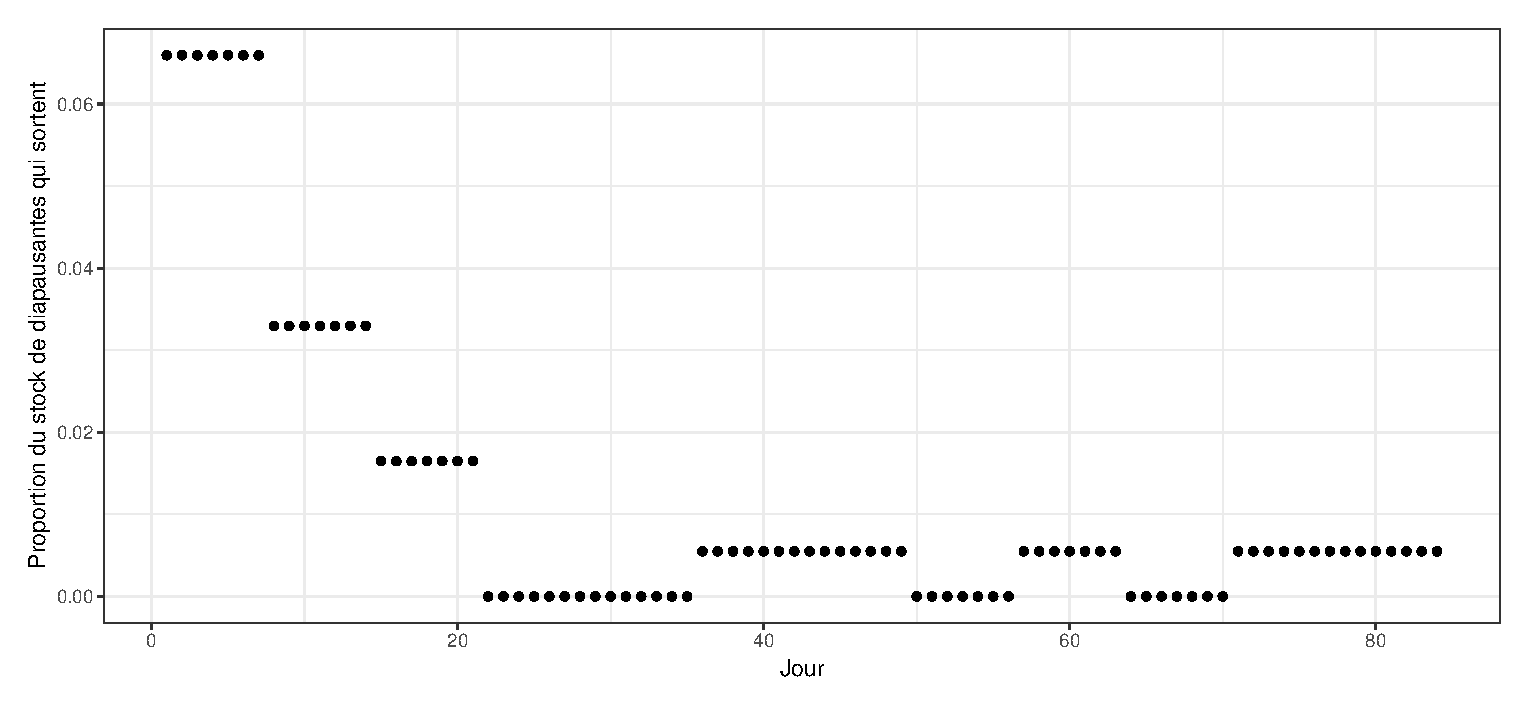
\epsfig{file = plots/sortie_diapause.eps, scale = 0.65}
 \caption{Proportion des individus en diapause qui sortent chaque jour}
 \label{sortie}
\end{figure}

\paragraph{4.} Identifier la date de début d'émergence des diapausantes. Il semblait y avoir un seuil vers 20.5\textdegree C. Pour l'année 2017, le seuil est atteint au 15ème jour, à savoir le 2 août.

\paragraph{5.} À partir de là, il ne reste plus qu'à l'implémenter dans le modèle en rajoutant une variable \texttt{stock} à calibrer autour de 15615. Il faut veiller à séparer $\mu_{\text{MS}}^1$ de 
$\mu_{\text{MS}}^2$ et d'appliquer le sex-ratio à tous les individus qui sortent du sol.

\section*{Résultats}

La calibration de la variable \texttt{stock} s'est faite autour de 15615, en prenant une marge d'environ 30\%. Pour être plus précis, on a choisi l'intervalle $[10900;20300]$.
Le modèle avec diapause, une probabilité de pupaison ajustée sur les températures sur la quinzaine donne les résultats visibles sur la figure~\ref{diap}.
\begin{figure}[ht]
 \centering
 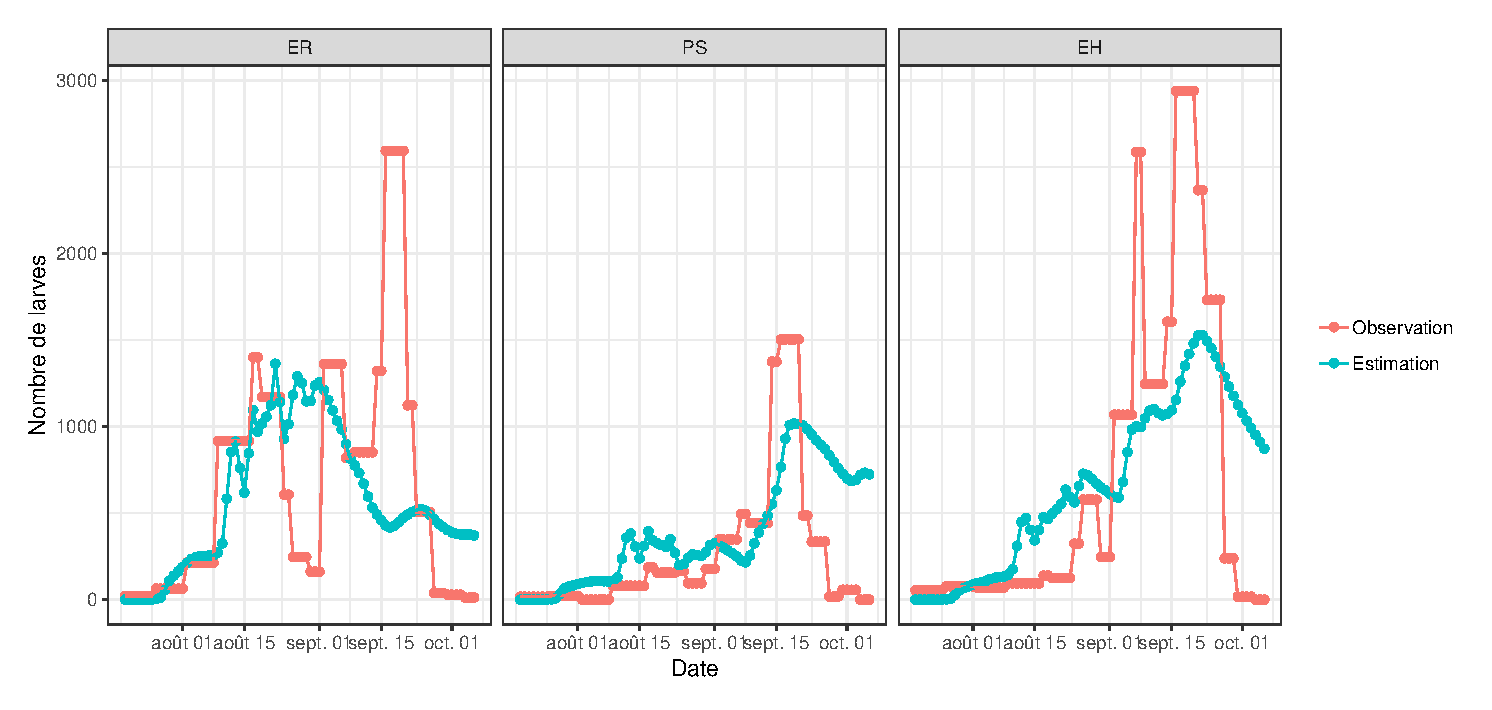
\epsfig{file = plots/with_diap.eps, scale = 0.65}
 \caption{Proportion des individus en diapause qui sortent chaque jour}
 \label{diap}
\end{figure}

Les paramètres utilisés sont 
\begin{center}
\begin{tabular}{llllll}
$\gamma$ & $p_m$ & $\mu_{\text{ER}}$ & $\mu_{\text{EH}}$ & $k$ & \texttt{stock}\\
0.048 & 0.986 & 0.815 & 0.167 & 0.150 & 6147
\end{tabular}
\end{center}

La fin de saison n'est toujours pas prise en compte dans la mesure où le phénomène qui la régit nous est pour l'instant inconnu.



\clearpage
\bibliography{p_pup}

\end{document}

